\documentclass[12pt]{article}

\usepackage{graphicx}
\usepackage{epstopdf}


\usepackage[spanish]{babel} % silabea palabras castellanas <- Puedo poner comentarios para explicar de que va este comando en la misma línea
\selectlanguage{spanish} 

%Encoding
\usepackage[utf8]{inputenc} % Acepta caracteres en castellano
\usepackage[T1]{fontenc} % Encoding de salida al pdf

%Triunfó el mal
\usepackage[normalem]{ulem}
\useunder{\uline}{\ul}{}
\providecommand{\e}[1]{\ensuremath{\times 10^{#1}}}
\usepackage{quotmark} %Uso consistente con la RAE de comillas
\usepackage{listings} % Comandos de la terminal

\usepackage{textcomp}
\usepackage{gensymb}


%Hipertexto
\usepackage[colorlinks=true,urlcolor=blue,linkcolor=blue]{hyperref} % navega por el doc: hipertexto y links

%Aquello de las urls
\usepackage{url} 

%simbolos matemáticos
\usepackage{amsmath}
\usepackage{amsfonts}
\usepackage{amssymb}
\usepackage{physics} %Best pack

% permite insertar gráficos, imágenes y figuras, en pdf o en eps
\usepackage{graphicx}
\usepackage{epstopdf}
\usepackage{multirow}
\usepackage{float}
\usepackage[export]{adjustbox}
% geometría del documento, encabezados y pies de páginas, márgenes
\usepackage[left=2cm, right=5cm, top=2cm]{geometry}
%\geometry{letterpaper,left=1mm}
\usepackage{comment}

%\usepackage[english]{babel}
%\usepackage[latin5]{inputenc}
% \usepackage{hyperref}
%\newdate{date}{10}{05}{2013}
%\date{\displaydate{date}}
\usepackage{setspace} 
\onehalfspacing
%\setlength{\parindent}{4em}
\setlength{\parskip}{1em}
\renewcommand{\baselinestretch}{2.0}
\begin{document}
\title{Cúmulos Abiertos \\ Taller 9: Búsqueda de estrellas variables}

\author{
\textbf{Javier Alejandro Acevedo Barroso\thanks{e-mail: \texttt{ja.acevedo12@uniandes.edu.co}}}\\
\textit{Universidad de los Andes, Bogotá, Colombia}\\
 }% Hasta aquí llega el bloque "author" (son dos autores por informe, orden alfabético)

\date{\today}
%\date{Versión $\alpha \beta$ fecha del documento}
\maketitle %Genera el título del documento


\normalsize
\newpage




\section{Catálogo de estrellas variables}
El objetivo de este ejercicio es la obtención de periodos para las curvas de luz y la correcta clasificación de estrellas variables de acuerdo al tipo de curva de luz. Para ello, nos valdremos del programa de software libre \tqt{FNPEAKS} escrito por Zbigniew Kołaczkowski en el \tqt{Instituto Astronómico de la Universidad de Breslavia} en Polonia. El programa FNPEAKS nos permite encontrar las frecuencias y periodos con mayor amplitud en el espacio de Fourier.
La metodología fue:
\begin{itemize}
\item Primero se reutilizó el análisis anterior en donde se segregó las candidatas a estrellas variables y se les separó en un archivo, se tomó la misma función (un polinomio de grado 13) que en el ejercicio anterior, pero se varió el Threshold para obtener cada vez un mayor número de estrellas candidatas.
\item Una vez obtenidas la lista de candidatas, se descartó las candidatas con \emph{menos} de 20 observaciones.
\item A la lista de candidatas final se le aplicó FNPEAKS, y se tomó únicamente las estrellas con algún periodo mayor o igual a 2 días.
\item A cada estrella seleccionada se le realizó una inspección manual a su curva de luz usando el periodo obtenido con FNPEAKS. Para ello se utilizó la tarea \tqt{PDM} de \tqt{IRAF} y se estudó posibles periodos alternativos.
\item Finalmente, se clasificó a la estrella de acuerdo a su periodo y su curva de luz.
\end{itemize}

La sintaxis de FNPEAKS es:
\begin{lstlisting}[language=bash]
$ ./fnpeaks estrella.dat frecuenciaMinima frecuenciaMaxima tamanoDelPaso
\end{lstlisting}
Donde se utilizó como frecuencia mínima 0.001(1/días), de modo que el periodo máximo de búsqueda fue 1000 días. Para frecuencia máxima se utilizó 100(1/días), objetivamente hablando el valor correcto de frecuencia máxima depende de la frecuencia con la que se toma los datos, sin embargo, se tomó hasta 100 por ser un ejercicio pedagógico y también para delimitar fuertemente el número de candidatas. Tomar una frecuencia máxima grande introduce bastantes picos a alta frecuencia, dado que esos picos de alta frecuencia serán descartados en el procesamiento posterior,  eso lleva a que solo los picos más grandes de frecuencia baja (que son los que nos interesa) sean considerados. Así, cada estrella señalada por los scripts de ser una estrella variable, será casi seguramente una estrella variable. POr último, se usó un tamaño del paso de 0.0001.

El threshold inicial fue de 3, con el cual FNPEAKS solo encontró 3 estrelals variables con periodos mayores a 3 días. Finalmente se fijó un threshold de 2.6 en el cual se obtuvo 7 estrellas variables.



\begin{table}[htb]
    \centering
    \label{tabla}
	\begin{tabular}{|c|c|c }
	\hline
	3.WFI.dat & 53.19149 & binaria \\
	877.WFI.dat & 41.58004 & cefeida\\
	1950 & 14.437529 & cefeida \\
	4.WFI.dat & 3.04553  & cefeida  \\
	201920.WFI.dat & 4.5527 & cefeida \\
	205515.WFI.dat & 3.44768 &cefeida \\
	1932.WFI.dat & 3.88651 & cefeida\\
\hline
	\end{tabular}
\end{table}


A contiación se presentan las curvas de luz obtenidas más \tqt{bonitas}. Los scripts utilizados están en los anexos finales.




\begin{figure}[H]
  \centering
   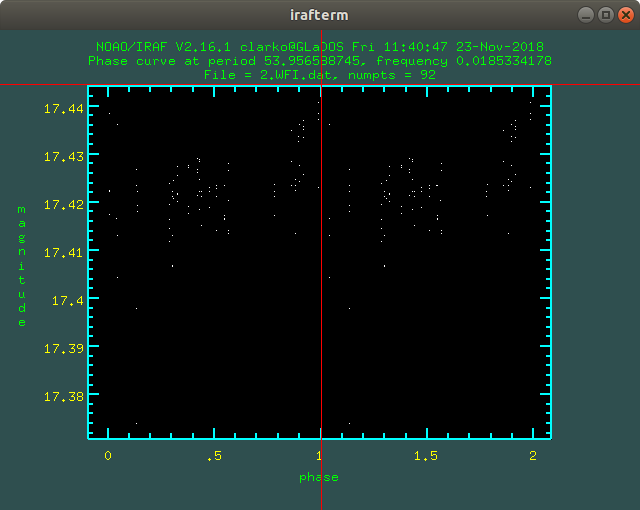
\includegraphics[scale = 0.5]{2.png}
  \caption{En la estrella 2 WFI se observa un pico bajo y un pico alto, típico de una estrella binaria eclipsante con un periodo de ~54 días.}
  \label{figura}
\end{figure}

\begin{figure}[H]
  \centering
   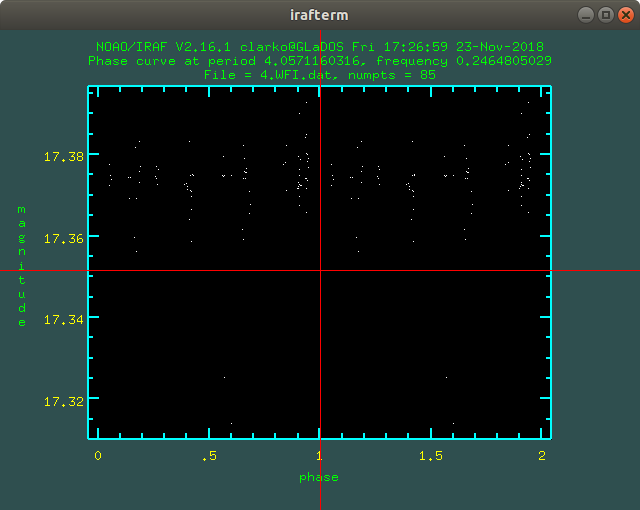
\includegraphics[scale = 0.5]{4.png}
  \caption{En la estrella 4 WFI se observa picos de más o menos la misma intensidad y un ocasional pico más alto, esto apunta a que es una estrella cefeida con de pronto una compañera eclipsante (aunque lo más probable es solo cefeida).}
  \label{figura}
\end{figure}

\begin{figure}[H]
  \centering
   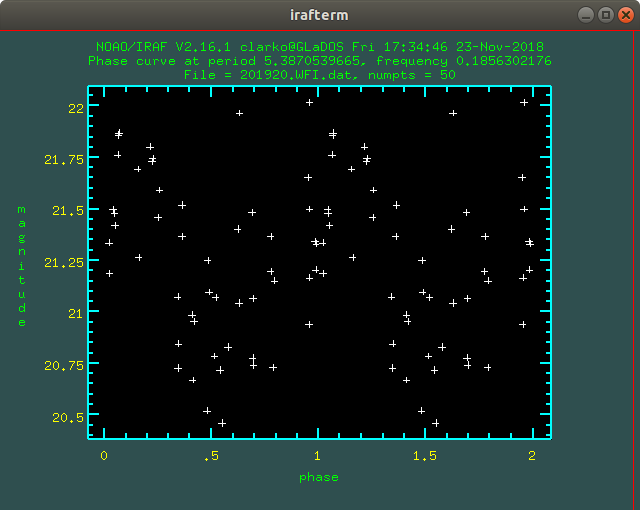
\includegraphics[scale = 0.5]{201920.png}
  \caption{En la estrella 201920 WFI se observan dos únicos picos de más o menos igual intensidad. Esto apunta  a una variable cefeida.}
  \label{figura}
\end{figure}

\begin{figure}[H]
  \centering
  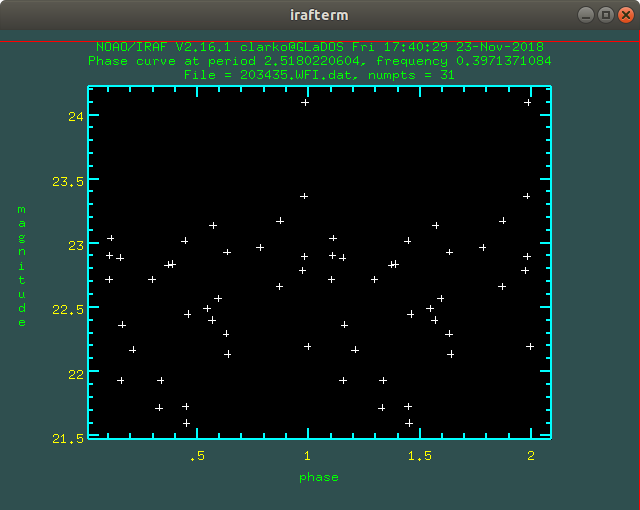
\includegraphics[scale = 0.5]{203435.png}
  \caption{En la estrella 203435 WFI se observa dos picos de más o menos igual intensidad. Esto apunta  a una variable cefeida.}
  \label{figura}
\end{figure}




%\bibliography{bibte}
\bibliographystyle{plain}


\section{Anexo}
Se usó 2 scrips de python y uno de bash para generar la lista de candidatas con sus periodos más probables. 

\begin{lstlisting}[language=bash]
$ ./tareaPeriodos.sh
\end{lstlisting}





\end{document}




\begin{figure}[H]
  \centering
   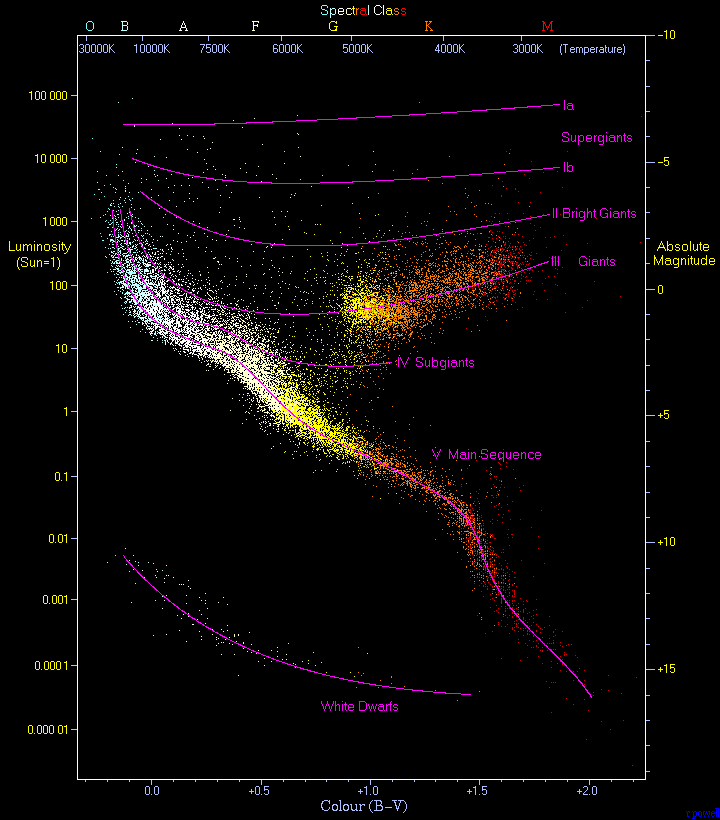
\includegraphics[width= 3.60in]{HRdiag.png}
  %\caption{Diagrama HR de 22000 estrellas del catálogo HIPPARCOS.\cite{hrdiag}  }
  \label{diag}
\end{figure}



\begin{table}[htb]
    \centering
    \label{tabla}
	\begin{tabular}{|c|c|c|c|c| }
	\hline
	Cúmulo & $E(B-V)$ & $m-M$ & Distancia [$pcs$] & Edad del cúmulo [millones de años]  \\ \hline
	NCG 752 & -0.03 & 8.02 & 401.79 & 1259  \\ \hline
	Mel 20 & +0.09 & 6.35 & 186.2 & 63  \\ \hline
	M45 & +0.04 & 5.50 & 125.89 & 126  \\ \hline
	Hyades & 0.00 & 2.84 & 36.98 & 891  \\ \hline
	M44 & +0.04 & 6.21 & 174.58 & 794  \\ \hline
	M67 & -0.03 & 9.32 & 731.14 & 5623  \\ \hline
	IC 4665 & 0.18 & 7.86 & 373.25 & 224  \\ \hline
	M39 & +0.01 & 6.87 & 238.78 & 447  \\ \hline
	\end{tabular}
\end{table}

\begin{table}[htb]
	\begin{tabular}{|c|cccccccccccccccc| }
	\hline
	Tareas $\backslash$ Semanas & 1 & 2 & 3 & 4 & 5 & 6 & 7 & 8 & 9 & 10 & 11 & 12 & 13 & 14 & 15 & 16  \\
	\hline
	1 & X & X & X  &   &   &   &   &  &  &   &   &   &   &   &   &   \\
	2 &   &  & X & X & X &  &  &   &   &  &  &  &   &  &  &   \\
	3 &   &   &   &  & X  & X  & X  & X &   &   &   &  &   &   &  &   \\
	4 &  &  &  &  &  &  &  & X & X & X & X &   &   &   &   &   \\
    5 &  &  &  &  &  &  & X & X &  &  &  &   &   &   &   &   \\
	6 &   &   &   &   &  &   &  X & X  &  &   &  X & X &  X & X  & X &   \\
	\hline
	\end{tabular}
\end{table}
\vspace{1mm}
%CCDRED se encarga de la corrección en sí, sus parámetros son: el tipo de dato de los pixeles (real, short, etc), el nombre del backup (en caso de querer un backup), el archivo de traducción del instrumento (que para una CCD estandar ya viene incluido en IRAF
